\documentclass{beamer}
\usetheme{Pittsburgh}
\beamertemplatenavigationsymbolsempty


\usepackage{amsmath}
\usepackage{amssymb}
\usepackage{bm} % For bold math symbols
\usepackage{graphicx}
\usepackage{tikz}



\usepackage{subfig} % Changed from subfigure (deprecated)
\usepackage{multirow}
\usepackage{multicol}
\usepackage{color}
\usepackage{url}
\usepackage{hyperref}
\usepackage{listings}
\usepackage[noend]{algorithm}
\usepackage{physics} 
% add image path
\graphicspath{{../Images/}}






\DeclareMathOperator{\argmin}{argmin}
\DeclareMathOperator{\argmax}{argmax}






\title{Weekly Updates\\
\tiny{Wednesday, 12/03/2025}}
\author{Andrea Bonifacio}
\date{}

\begin{document}

\begin{frame}
\titlepage
\end{frame}


\begin{frame}{Neural Modes Paper - Critical Review}
    \begin{itemize}
        \item After implementing both StVenant-Kirchhoff and Neo-Hookean materials, I realized that this method works well for small deformations.
        \item Most of the deformation is already captured by the linear modes (the nonlinear correction is small, around 1\%).
        \item I am having problem with changing the material properties during the simulation.
    \end{itemize}
\end{frame}


\begin{frame}
    \frametitle{Network Architecture}
    \begin{itemize}
        \item The network is a feedforward neural network.
        \item The input is the modal coordinate \( z \in \mathbb{R}^m \).
        \item The output is a correction on the displacement field \( \mathbf{y} \in \mathbb{R}^n \).
    \end{itemize}



\begin{center}
        
        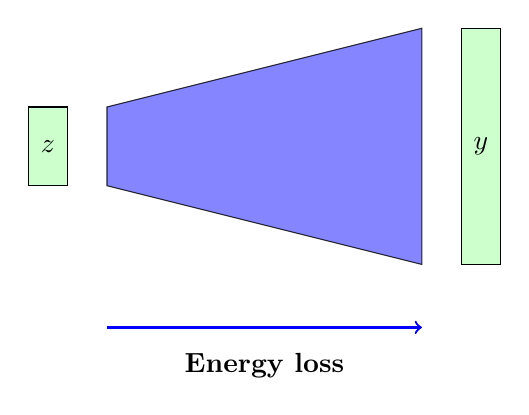
\begin{tikzpicture}
            % Modal coordinate (z)
            \draw[fill=green!20] (-3, 1) rectangle (-2.5,2);
            \node at (-2.75, 1.5) {$z$}; % Label inside the rectangle
            
            % Displacement (u)
            \draw[fill=green!20] (2.5,0) rectangle (3,3);
            \node at (2.75, 1.5) {$y$}; % Label inside the rectangle
            
            % Energy loss transition
            \draw[fill=blue!60,opacity=0.8] (-2,1) -- (2,-0) -- (2,3) -- (-2,2) -- cycle;
            \node[below] at (0,-1) {\textbf{Energy loss}};
            
            % Energy loss arrow
            \draw[thick,blue,->] (-2,-0.8) -- (2,-0.8);
        
        \end{tikzpicture}
\end{center}
    
\end{frame}

\begin{frame}
    \frametitle{Training the network}
    \begin{itemize}
        \item At each iteration, the network is trained on a batch of modal coordinates randomly selected.
        \item Four loss functions are used:
        \begin{itemize}
            \item Energy loss: \( E(X + l + y)\), where \(X\) is the rest position, \(l\) is the linear mode given by \(z\) and \(y\) is the nonlinear correction.
            \item Orthogonality loss: \( y^T l = 0 \).
            \item Origin loss: \( y(0) = 0 \).
        \end{itemize}
        \item The network is trained by minimizing the weighted sum of these losses.
        \[
        \text{Loss} = \text{Energy } + \lambda_1 \text{Orthogonality } + \lambda_2 \text{Origin}
        \]
    \end{itemize}
\end{frame}

\begin{frame}
    \frametitle{Visualization}
    \begin{figure}
        \centering
        \includegraphics[scale=0.15]{Images/image.png}
        \caption{Nonlinear latent space.}
    \end{figure}
\end{frame}

\begin{frame}
    \frametitle{Dynamic simulation}
    I started implementing it, but the optimization problem takes too long to solve.
    \begin{itemize}
        \item The optimization problem is solved using the L-BFGS-B algorithm. (As in the paper)
        \item Each iteration takes around 3-4 seconds.
        \item Maybe another optimization algorithm could be used?
    \end{itemize}
    \begin{itemize}
        \item The non-linear correction can be computed by:
        \[
        z_{n+1} = \underset{z}{\argmin}  \frac{1}{2h^2} \norm{n(z) - 2u_n + u_{n-1}}^2_M + E(n(z))
        \]
        \item Here \(n(z)\) is the non-linear correction computed by the network, and \(M\) is the mass matrix.
    \end{itemize}
\end{frame}

\begin{frame}
    \frametitle{What now?}
    \begin{itemize}
        \item What is our goal?
        \item Are there similar methods? There are some papers on strain modes from the same authors.
        \item In the same paper they mention a Rotation-Strain decomposition. Could be useful?
        \item Learn how to do simulations correctly
    
    \end{itemize}
\end{frame}

% Q&A
\begin{frame}
    \begin{center}
        \color{blue} \Huge{Questions?}
    \end{center}

\end{frame}
\end{document}

